
\section{Signal extraction}
\label{sec:signal}
\subsection{Fit description}
\label{subsec:fitdes}
The signal yields of \LbLckkpi and \LbLcDs(\Dskkpi) are extracted using unbinned extended maximum 
likelihood fits to the distributions of the PV-constrained and $\Lc$ mass constrained invariant mass ($m$) and \Dsp mass is not constrained to the known value. 
For the signal channel the likelihood has the form
\begin{equation}
\lum = \frac{e^{-(N_{\rm S}+\sum_j N_{{\rm B}_j})}}{N!}\times \prod^{N}_{i=1}[N_{\rm S}P_{\rm S}(m_i)+\sum_j N_{{\rm B}_j}P_{{\rm B}_j}(m_i)]
\end{equation}
where $N$ is the total number of events, index $i$ run over all candidates. 
$N_k$ ($P_k(m)$) is the yield (probability density function) for the category $k$ as signal (S) and background (B$_j$) respectively. 
In addition to the combinatorial background, 
there is also physics background, 
thus index $j$ accounts for different background sources. 


\subsection{Signal shape}
The signal shape for both channels is each modeled by the sum of two Crystal Ball (CB) functions~\cite{Skwarnicki:1986xj}. 
The pair of CB functions for each signal have a common mean. The general form of the signal shapes is:
\begin{equation}
\label{eq:Double_CB}
f_{sig} = f_{low} \times CB_-(m_0, \sigma_-, \alpha_-, n) + (1-f_{low})CB_+(m_0, \sigma_+, \alpha_+, n)
\end{equation}
where $m_0$ is the shared mean value of the CB functions, 
$\sigma_{\pm}$ are the width of the CB functions, 
$\alpha_\pm$ and $n$ are parameters to describe the shape corresponding to the energy loss due to bremsstrahlung. 
And plus and minus signs suggest that the two CB have tails on opposite sides. 
With all parameters free, 
there are large correlations between the parameters. 
Fewer independent parameters are actually needed to describe the signal shapes well. 
$\alpha_\pm$ and $n$ are determined using the simulated signal decays 
that pass all the selection as used for real data as well as the correct TRUEID information. 
The fitted shapes are shown in Figure.~\ref{fig:MassFitMC_foralpha}, 
and the fit parameters are shown in Table~\ref{tab:MassFitMC_foralpha}, 
and these parameters will be fixed when we fit the data. 

\begin{figure}[!btp]
\centering
   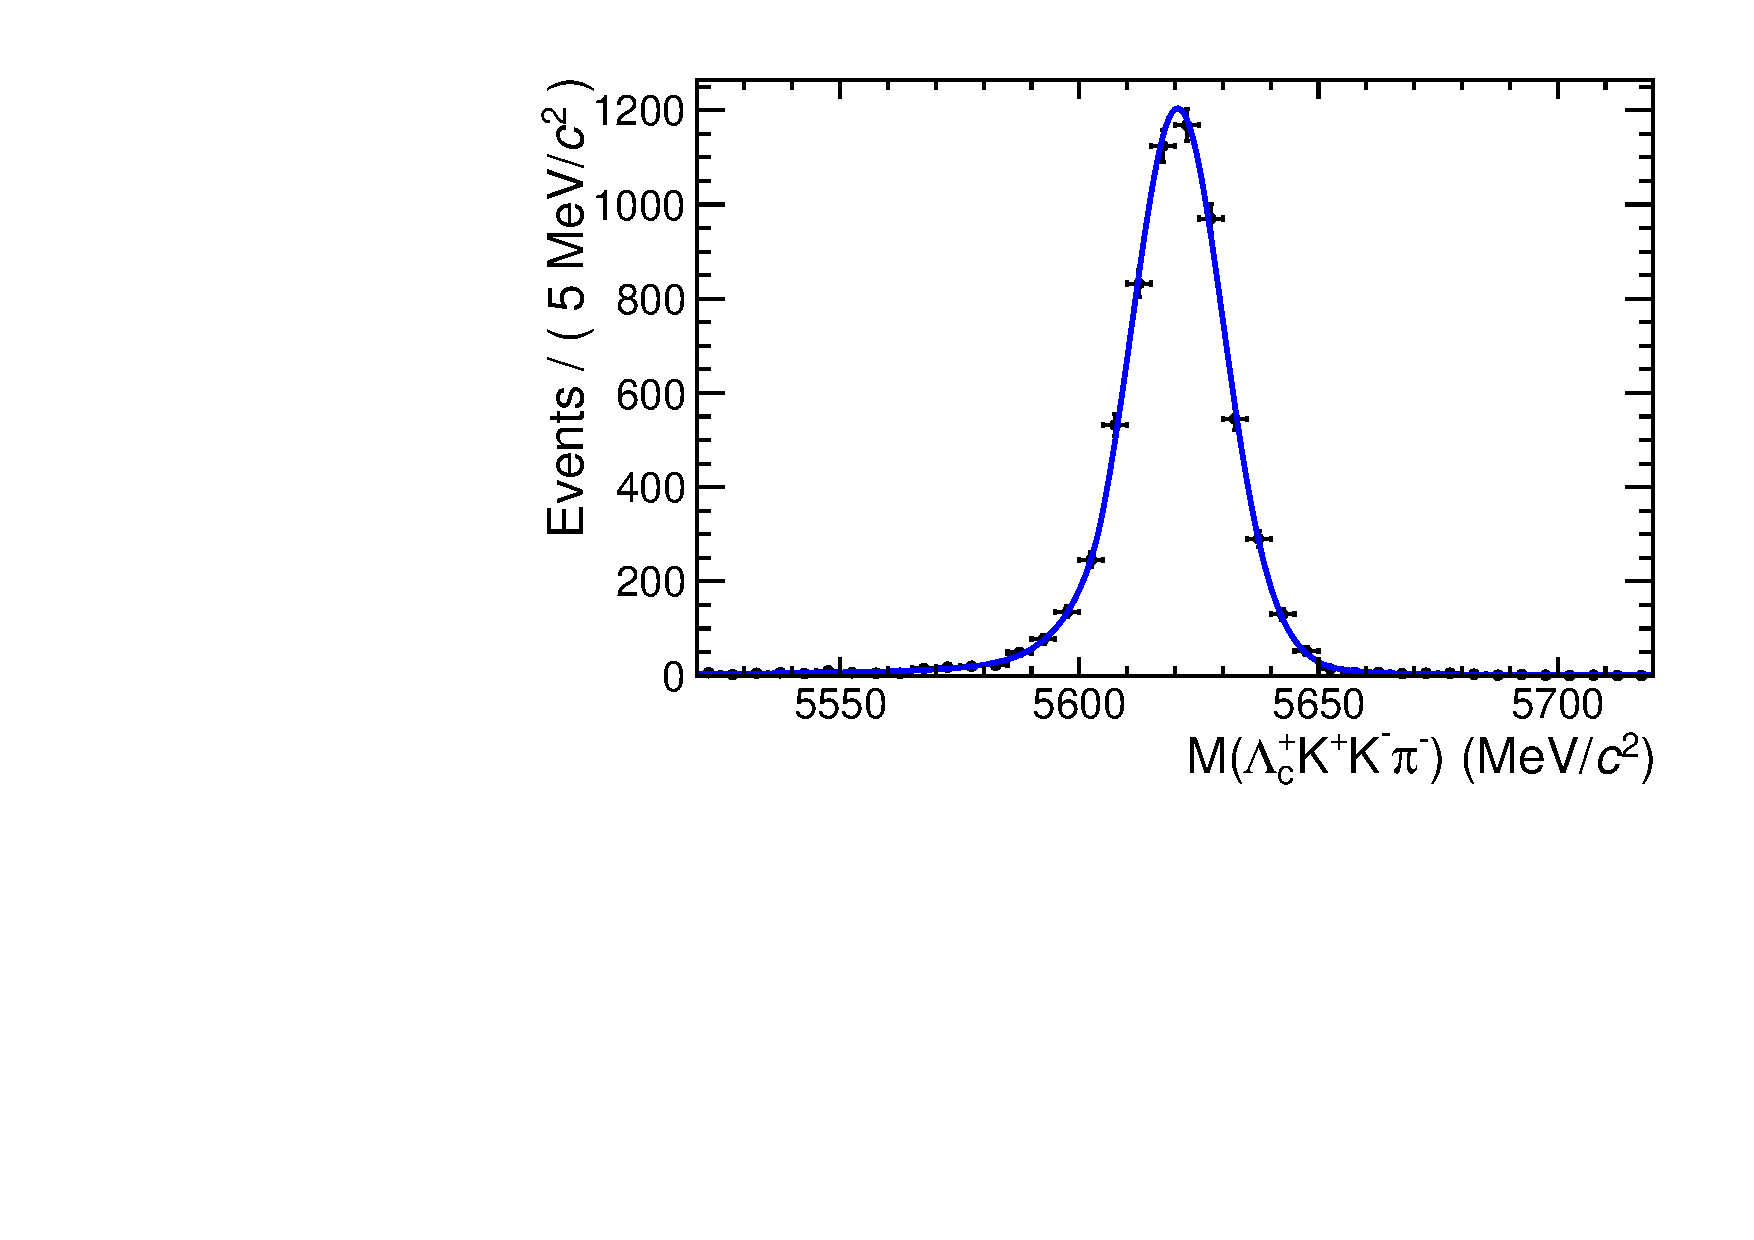
\includegraphics[scale=0.4]{Figures/05_open_charm/03_yiels/MC/Lb_LcKKPi.pdf}%
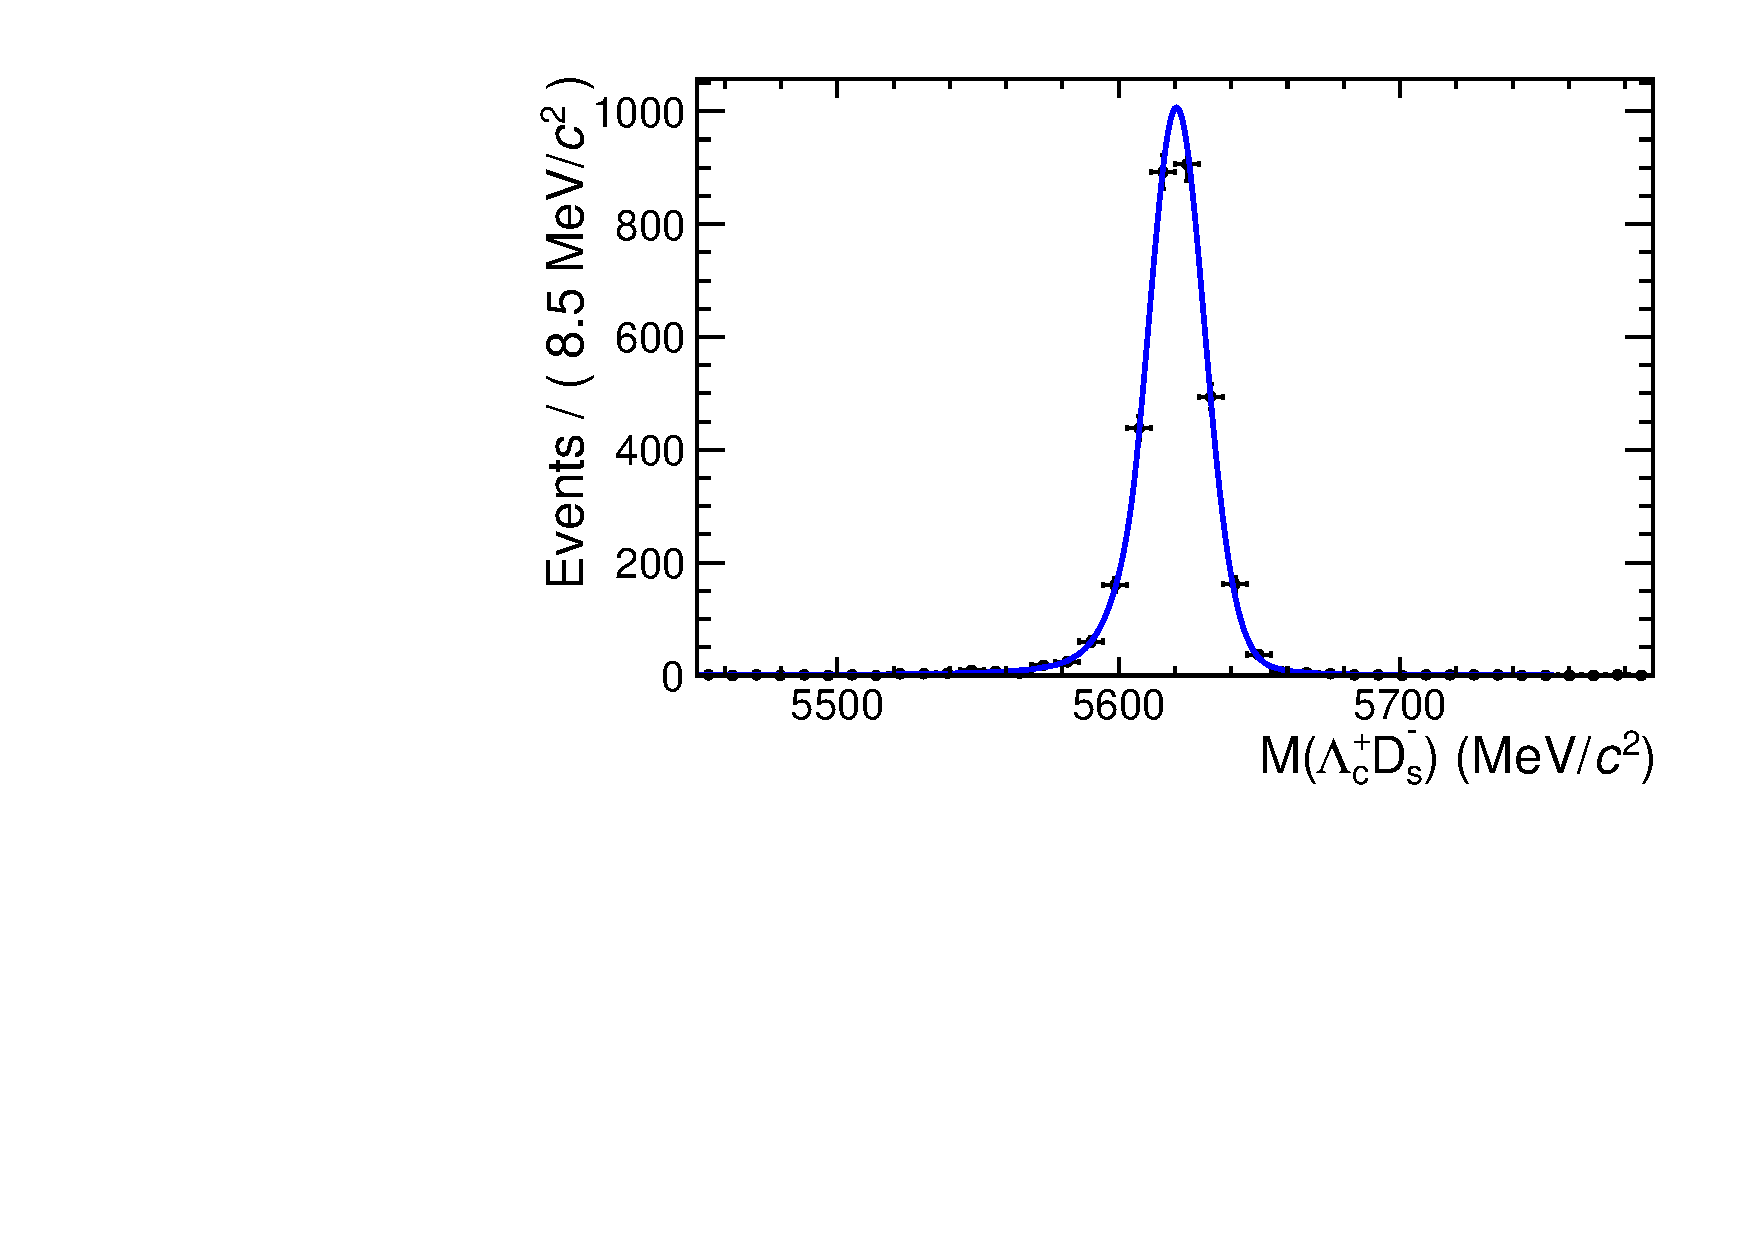
\includegraphics[scale=0.4]{Figures/05_open_charm/03_yiels/MC/Lb_LcDs.pdf}\\%
\caption{Signal shape for \LbLckkpi(left) and \LbLcDs(right) in the simulated events.}
\label{fig:MassFitMC_foralpha}
\end{figure}

\begin{table}[!bp]
\centering
	\caption{Fit result of simulated \LbLckkpi, \LbLcDs(\Dskkpi) mass spectrum}
\vspace{0.2cm}
\label{tab:MassFitMC_foralpha}
\begin{tabular}{c c c }\hline\hline
	Parameter&\LbLckkpi & \LbLcDs(\Dskkpi) \\\hline
$\alpha_+$& 1.8893$\pm$ 0.13594 		&1.5740  $\pm$ 0.26813\\
$\alpha_-$&-2.37242 $\pm$ 0.16725                &-2.11783 $\pm$ 0.31333 \\
$n$ &1.2957 $\pm$ 0.22705 			&2.4483  $\pm$ 0.61617\\
\hline
\end{tabular}
\end{table}

\subsection{Physics background}
\subsubsection{Background from $\Lb\to\Lc D_{s}^{*}$ in normalization channel}
The decay channel $\Lb\to\Lc D_{s}^{*}$ may emit a photon and be reconstructed as \LbLcDs, the shape of this background is obtained from $\Lb\to\Lc D_{s}^{*}$ simulated decays. The fitted shapes are shown in Figure~\ref{fig:MassFitMC_LcK}, and this histogram will be used when we fit the data sample.

\begin{figure}[!btp]
\centering
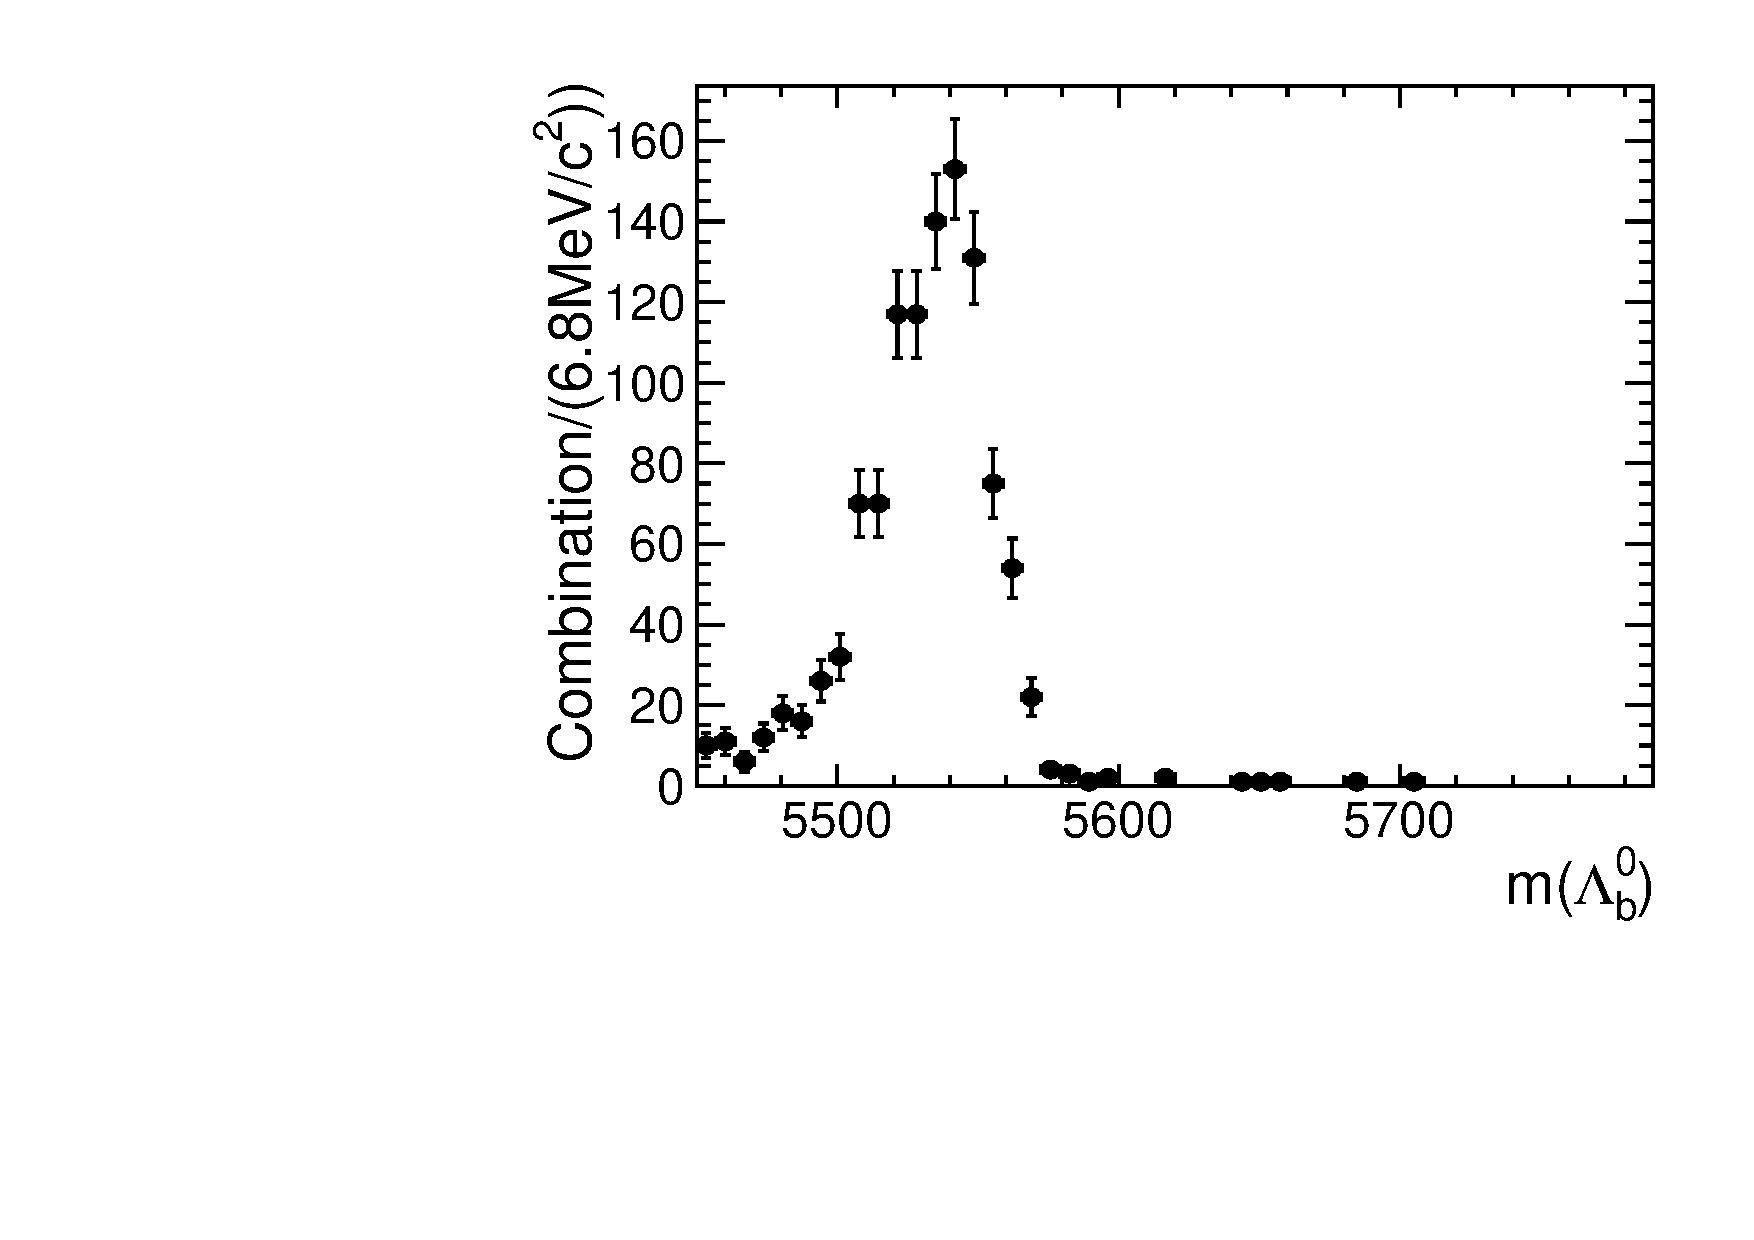
\includegraphics[scale=0.45]{Figures/05_open_charm/03_yiels/MC/physic_bkg.pdf}%
	\caption{Shape for $\Lb\to\Lc D_{s}^{*}$ reconstructed as \LbLcDs.}
\label{fig:MassFitMC_LcK}
\end{figure}


\subsubsection{\LbLckkpi background in normalization channel}
For \LbLcDs channel, 
there is a clear presence of \LbLckkpi in $D_s^-$ sideband, 
where the sideband the value of $|m(K^+K^-\pi^-)-m(\Ds)|$ changed from 40 to 80 \mev.(as shown in Figure.~\ref{fig:kkpi_bkg}) 
The width of this sideband is same to the $D_s^-$ mass window of $\pm40$ \mev, 
in order to gain the number of this background. 
This charmless background sizes and shapes will fixed in the mass fit. 
We also check this distribution in different sideband region and different \Ds life time regionse. 
More plots are in Appendix.~\ref{appendix:sideband} 

\begin{figure}[!btp]
\centering
   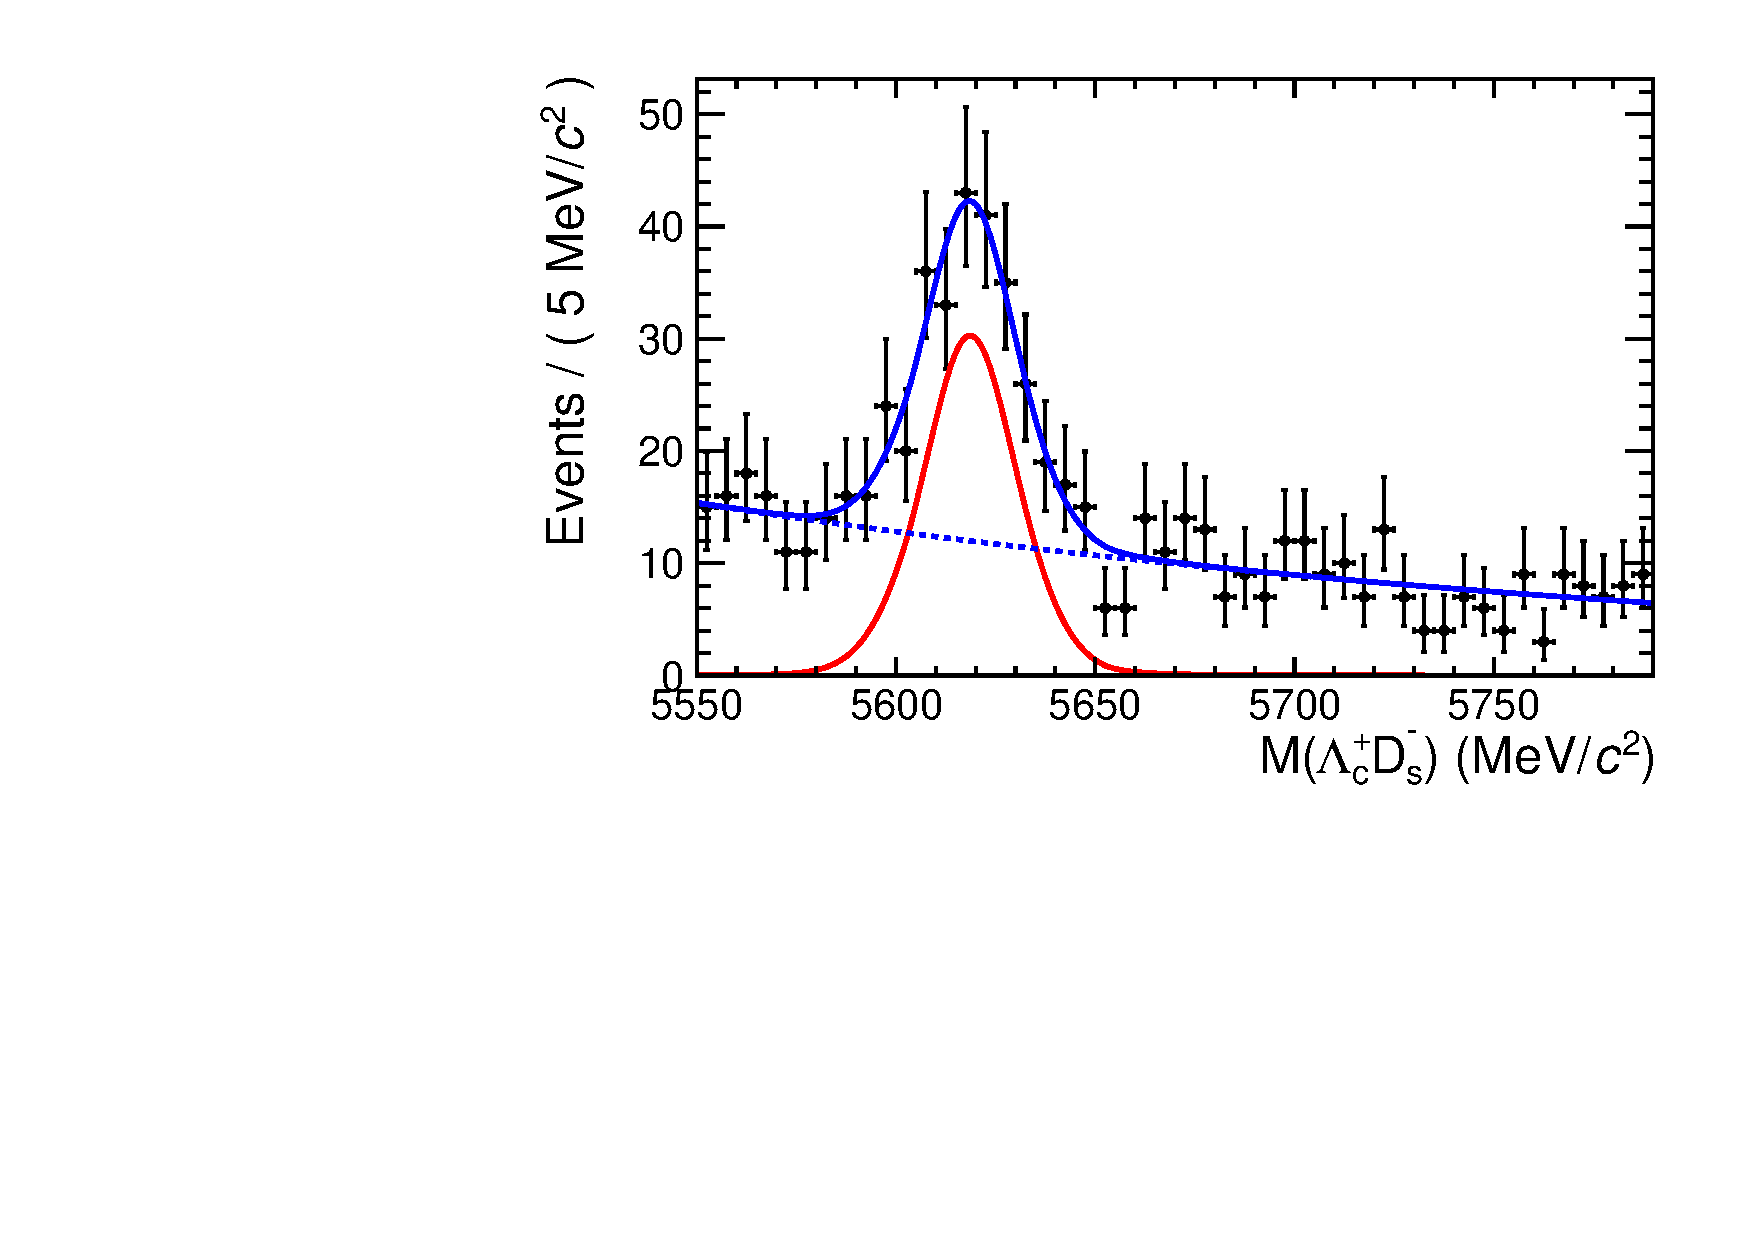
\includegraphics[scale=0.48]{Figures/05_open_charm/03_yiels/Data/LcDs_kkpi/Lb_LcDs.pdf}%
\caption{\LbLckkpi where the $KK\pi$ mass is in the sideband of the $D_s^-$. 
   The blue line is full fit, the blue dashed line is the combinatorial background, and the red line is the signal shape.}
\label{fig:kkpi_bkg}
\end{figure}


\subsubsection{$\Lb \to \Sigma_{c} K^+ K^- \pi^-$ background in signal channel}
For signal channel, 
there is a clear presence of $\Lb \to \Sigma_{c} K^+ K^- \pi^-$ in \LbLckkpi low sideband. 
The shape of this background is obtained from generator level simulated sample. 
Considering the mass resolution, 
we smear the \Lb candidate mass in the MC sample with 27.4\mevcc, 
which is the signal mass resolution estimated by fitting data sample. 
This background distribution is shown in Figure.~\ref{fig:sigma_bkg}.

\begin{figure}[!btp]
\centering
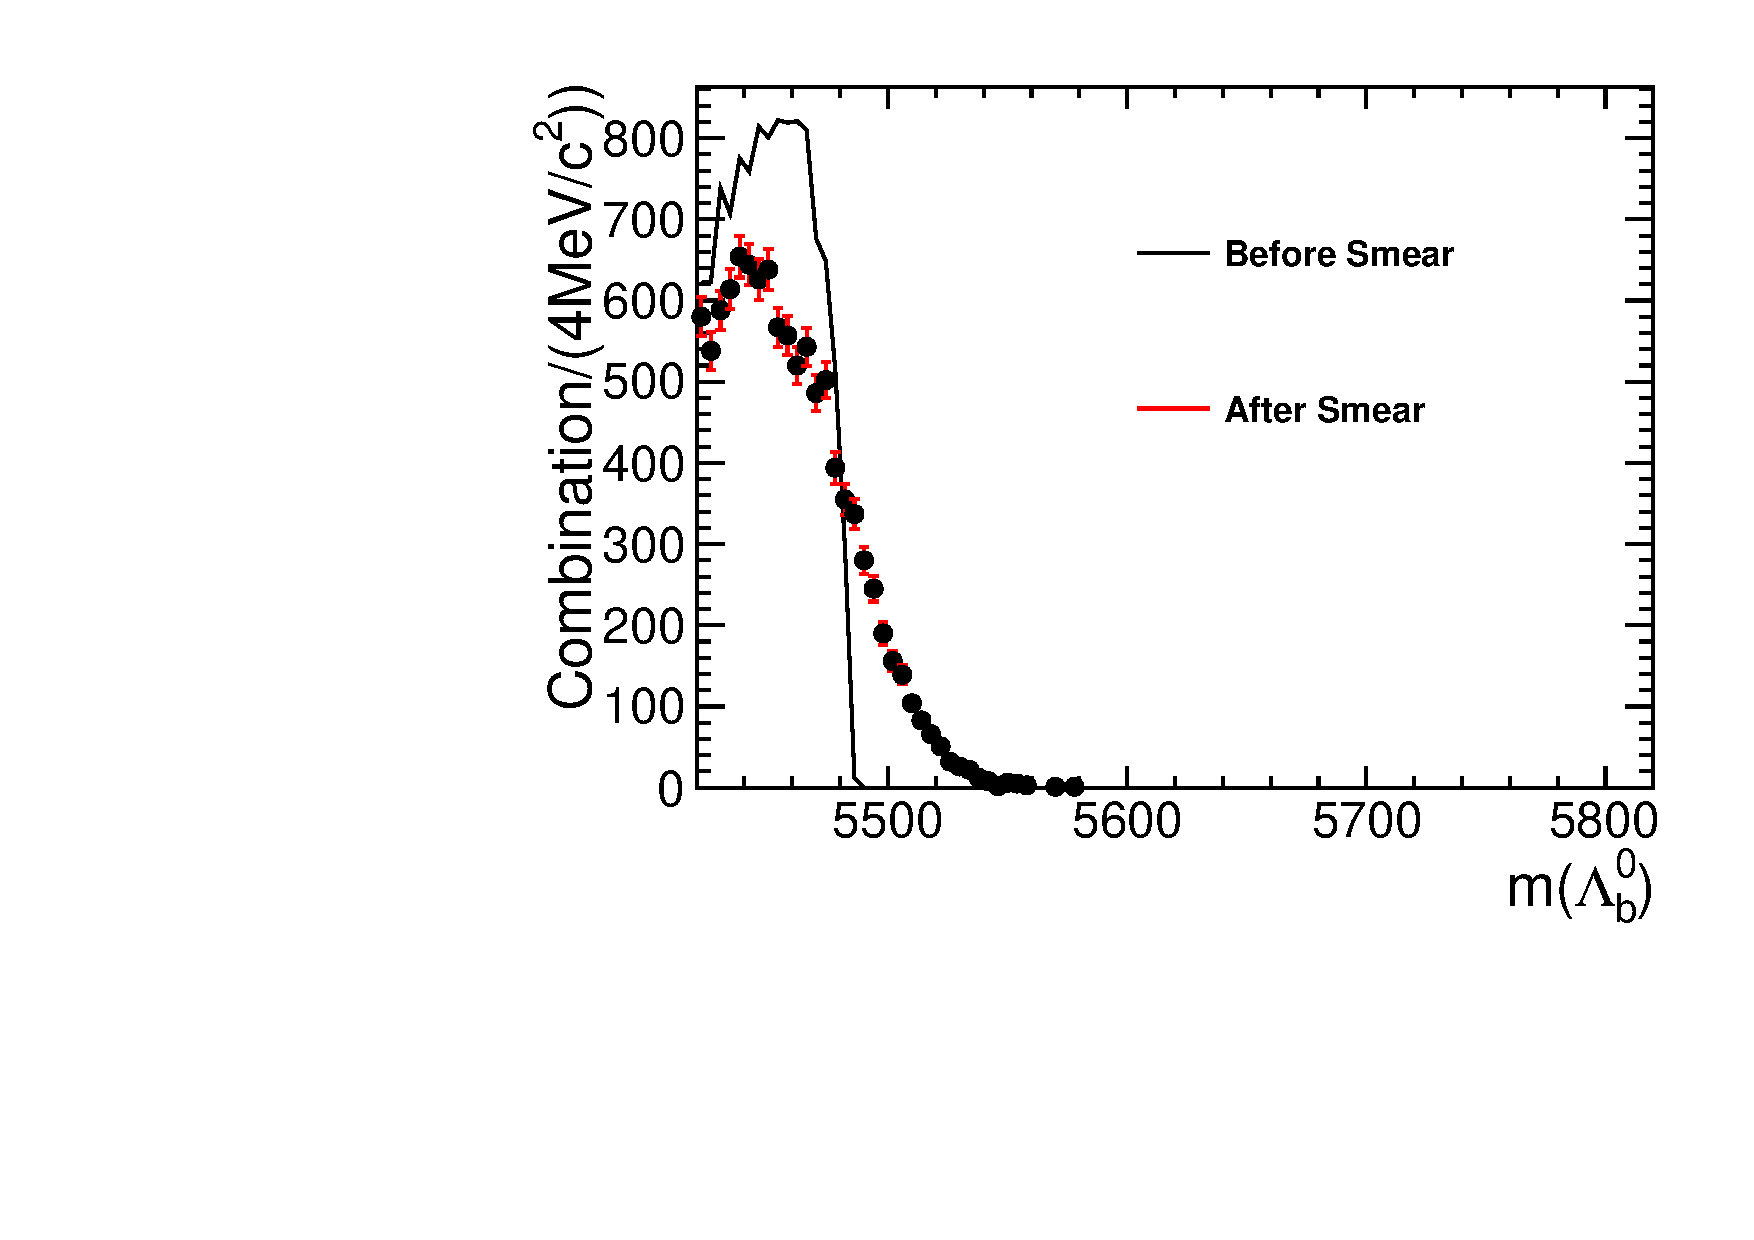
\includegraphics[scale=0.45]{Figures/05_open_charm/03_yiels/MC/Sigmakkpi/physic_bkg.pdf}%
\caption{ The distribution gained from $\Lb \to \Sigma_{c} K^+ K^- \pi^-$ MC sample. }
\label{fig:sigma_bkg}
\end{figure}


\subsection{Combinatorial background}
The combinatorial background shape is described by an exponential function, 
with a shape parameter that is freely varied in the fit.

\subsection{Fit results}
Unbinned maximum likelihood fits to the $\Lc\Kp\Km\pim$ and  $\Lc \Dsm$ mass spectra, 
with some parameters are fixed to the value obtained from Monto Carlo. 
The fit results for \LbLckkpi are shown in Figure.~\ref{fig:MassFit_LbLcpppi} and Table~\ref{tab:MassFit_LbLcpppi}. 
The fit results for \LbLcDs is shown in Figure.~\ref{fig:MassFit_LbLcpi} and Table~\ref{tab:MassFit_LbLcpi}. 
To reduce the number of free parameters, 
the ratio of $\sigma^+$ and $\sigma_-$ in \LbLcDs signal shape is fixed to the value obtained from the simulation. 


\begin{figure}[!btp]
\centering
   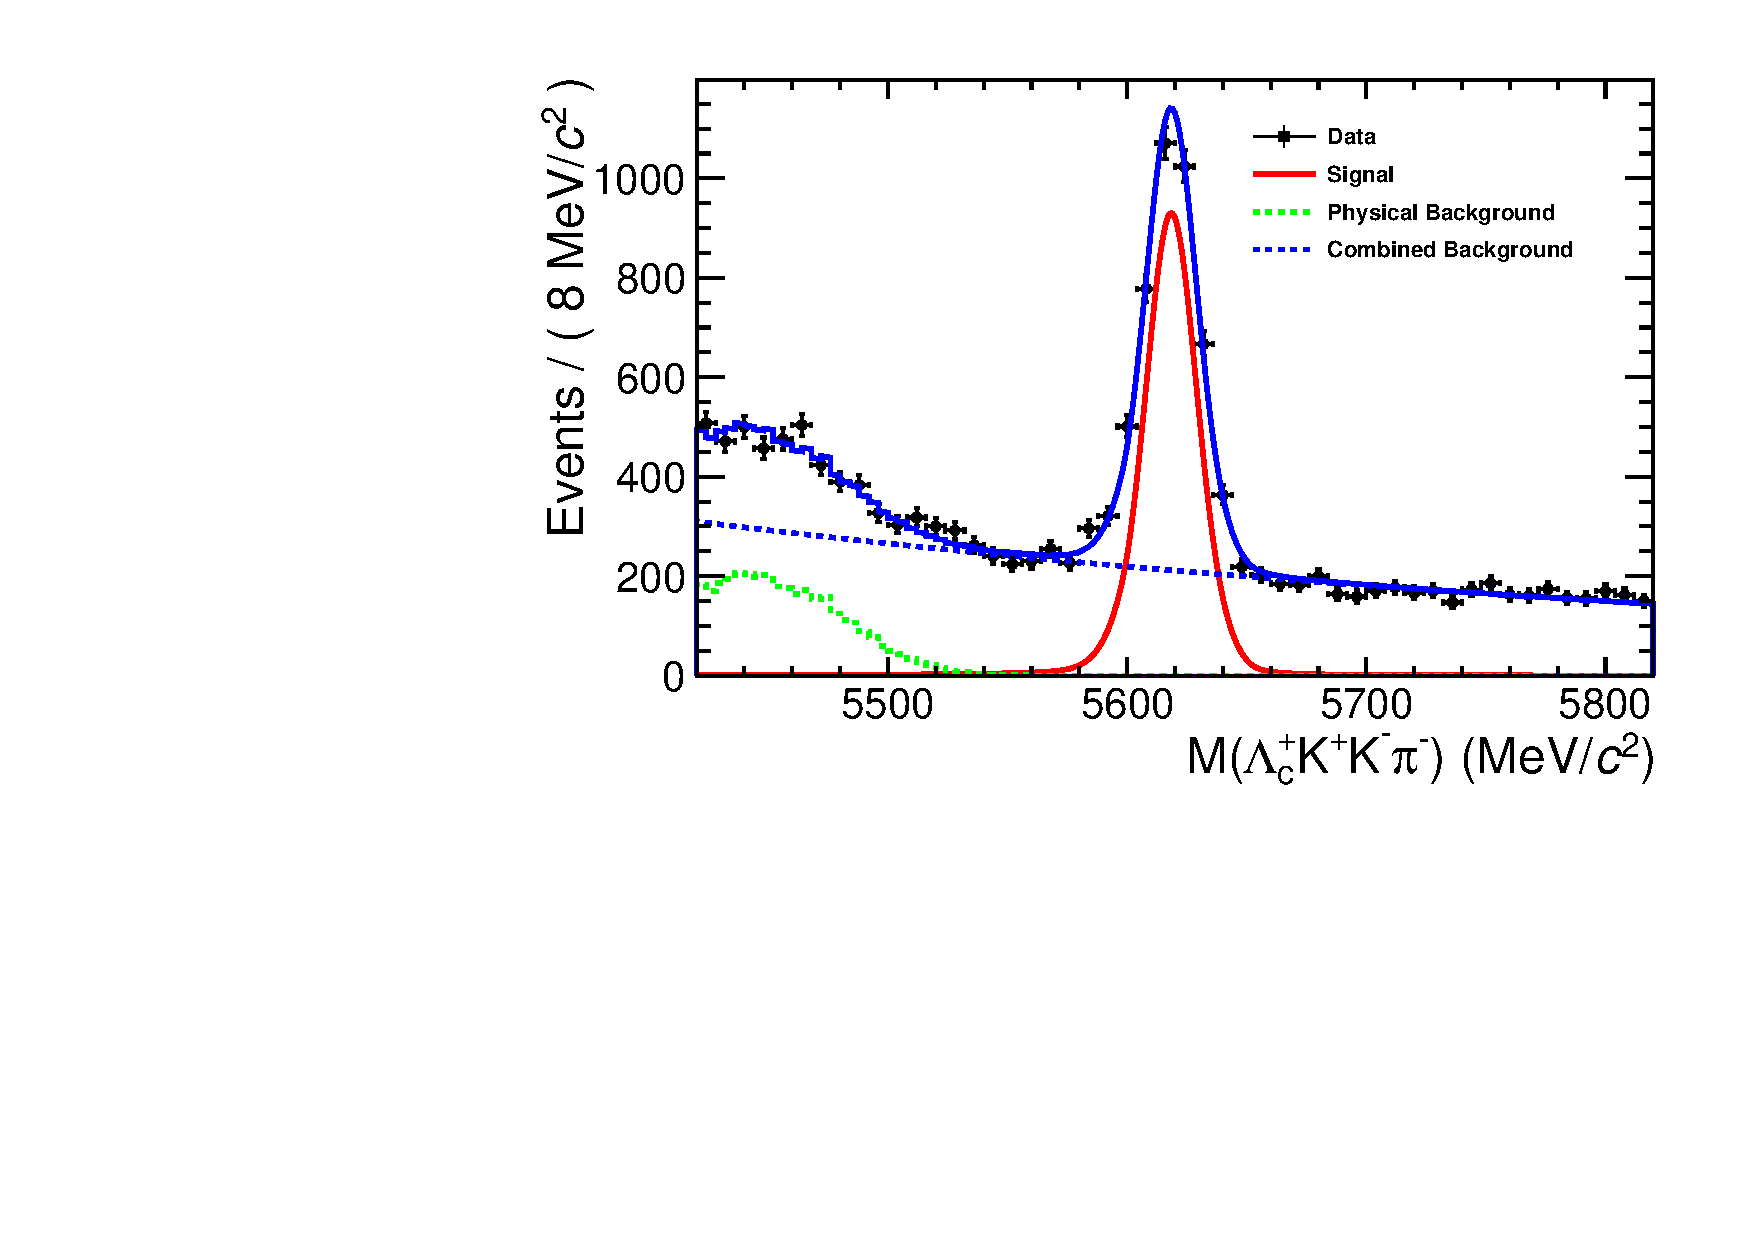
\includegraphics[scale=0.48]{Figures/05_open_charm/03_yiels/Data/Lb_KKPi_plot/Lb_LcKKPi.pdf}\\%
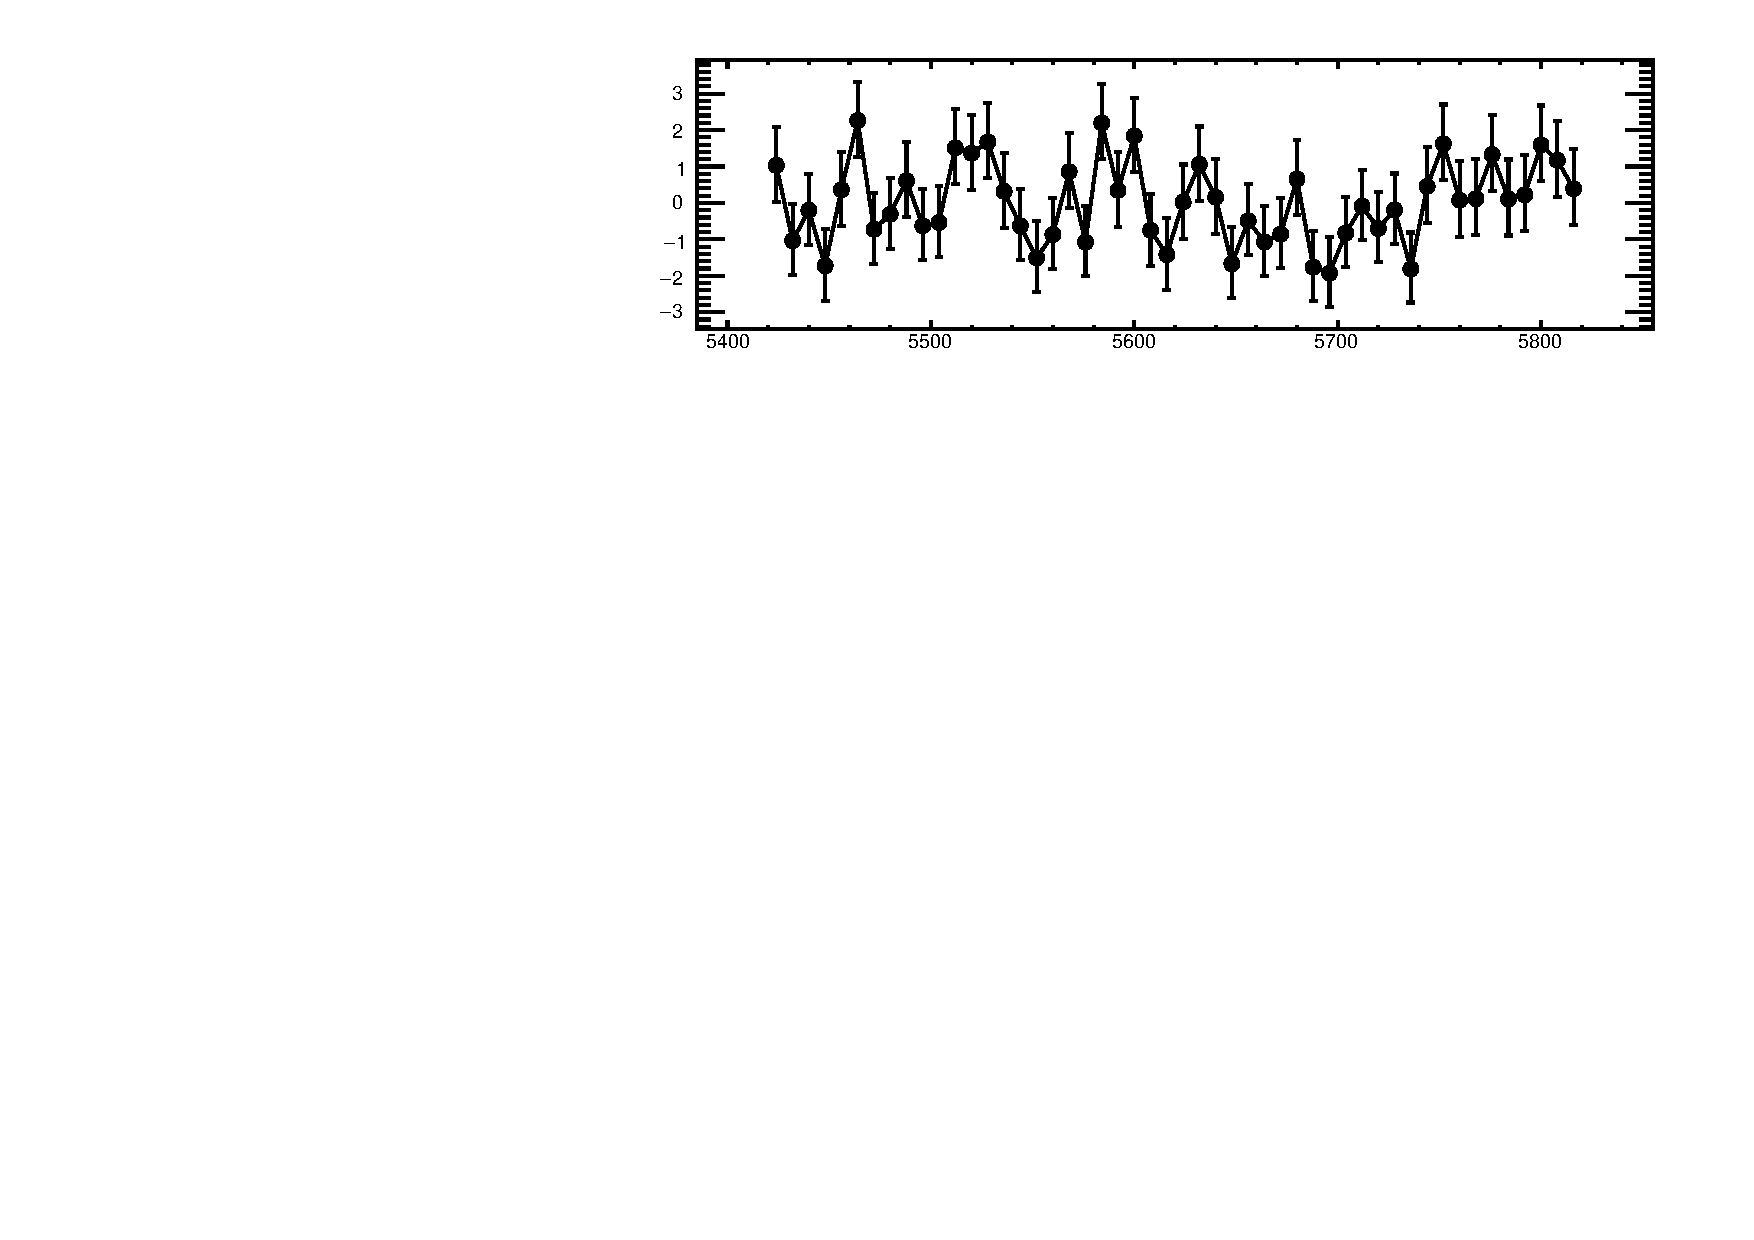
\includegraphics[scale=0.48]{Figures/05_open_charm/03_yiels/Data/Lb_KKPi_plot/Lb_LcKKPi_pull.pdf}%
	\caption{Reconstructed mass distribution for \LbLckkpi candidates. 
	A fit is overlaid, as described in the text. 
	The blue line is full fit, the blue dashed line is the combinatorial background, 
	the green dashed line is $\Lb \to \Sigma_{c} K^+ K^- \pi^-$ background and the red dashed line is the signal shape.}
\label{fig:MassFit_LbLcpppi}
\end{figure}


\begin{table}[!btp]
\centering
\caption{Fit result of \LbLckkpi mass spectrum in data sample.}
\vspace{0.2cm}
\label{tab:MassFit_LbLcpppi}
\begin{tabular}{c c }\hline\hline
Parameter& Value \\\hline
$m_0$ (MeV/$c^2$)& 5618.5 $\pm$  0.3 \\
$n_{sig}$     & 3411.0 $\pm$ 75.5\\
$n_{phy bkg}$ & 1672.4 $\pm$ 26.3\\
\hline\hline
\end{tabular}
\end{table}


\begin{figure}[!btp]
\centering
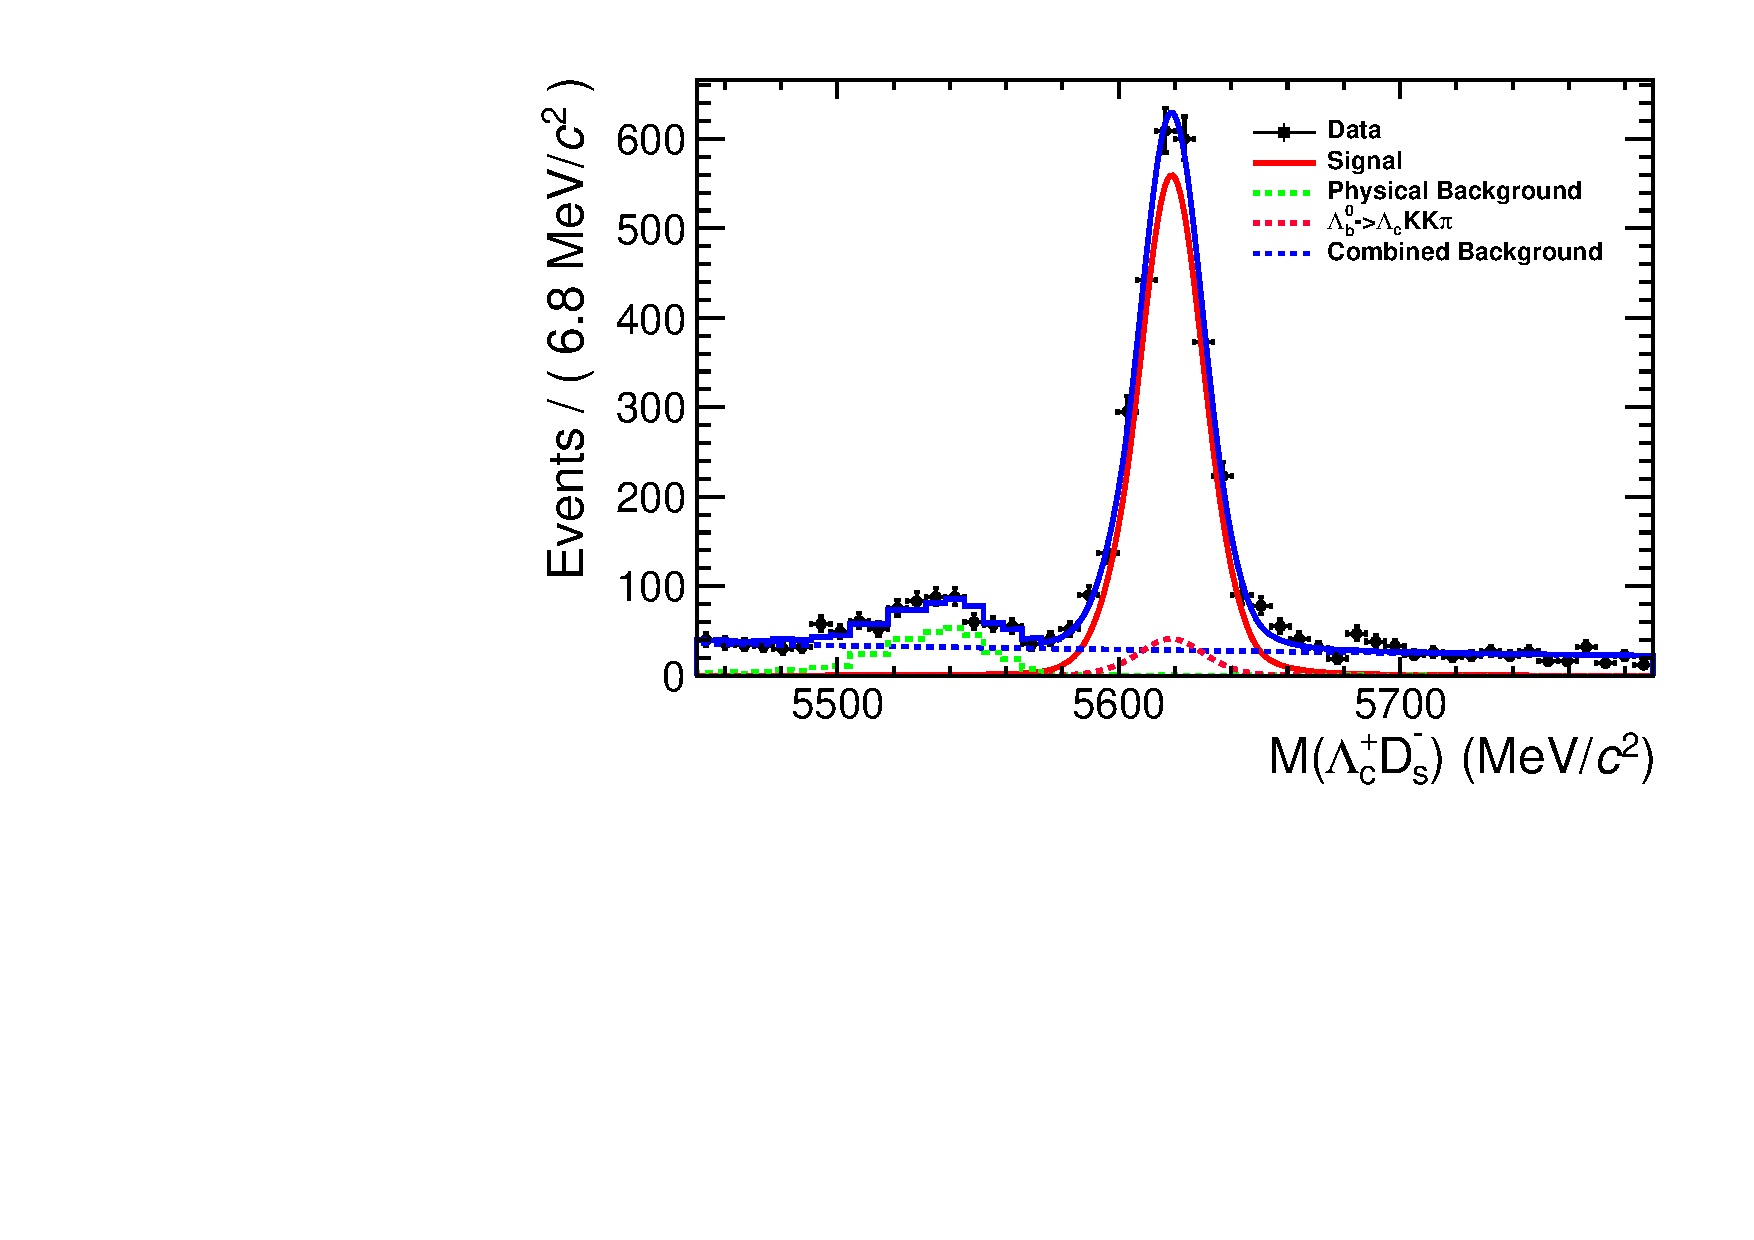
\includegraphics[scale=0.48]{Figures/05_open_charm/03_yiels/Data/Lb_LcDs_plot/Lb_LcDs.pdf}\\%
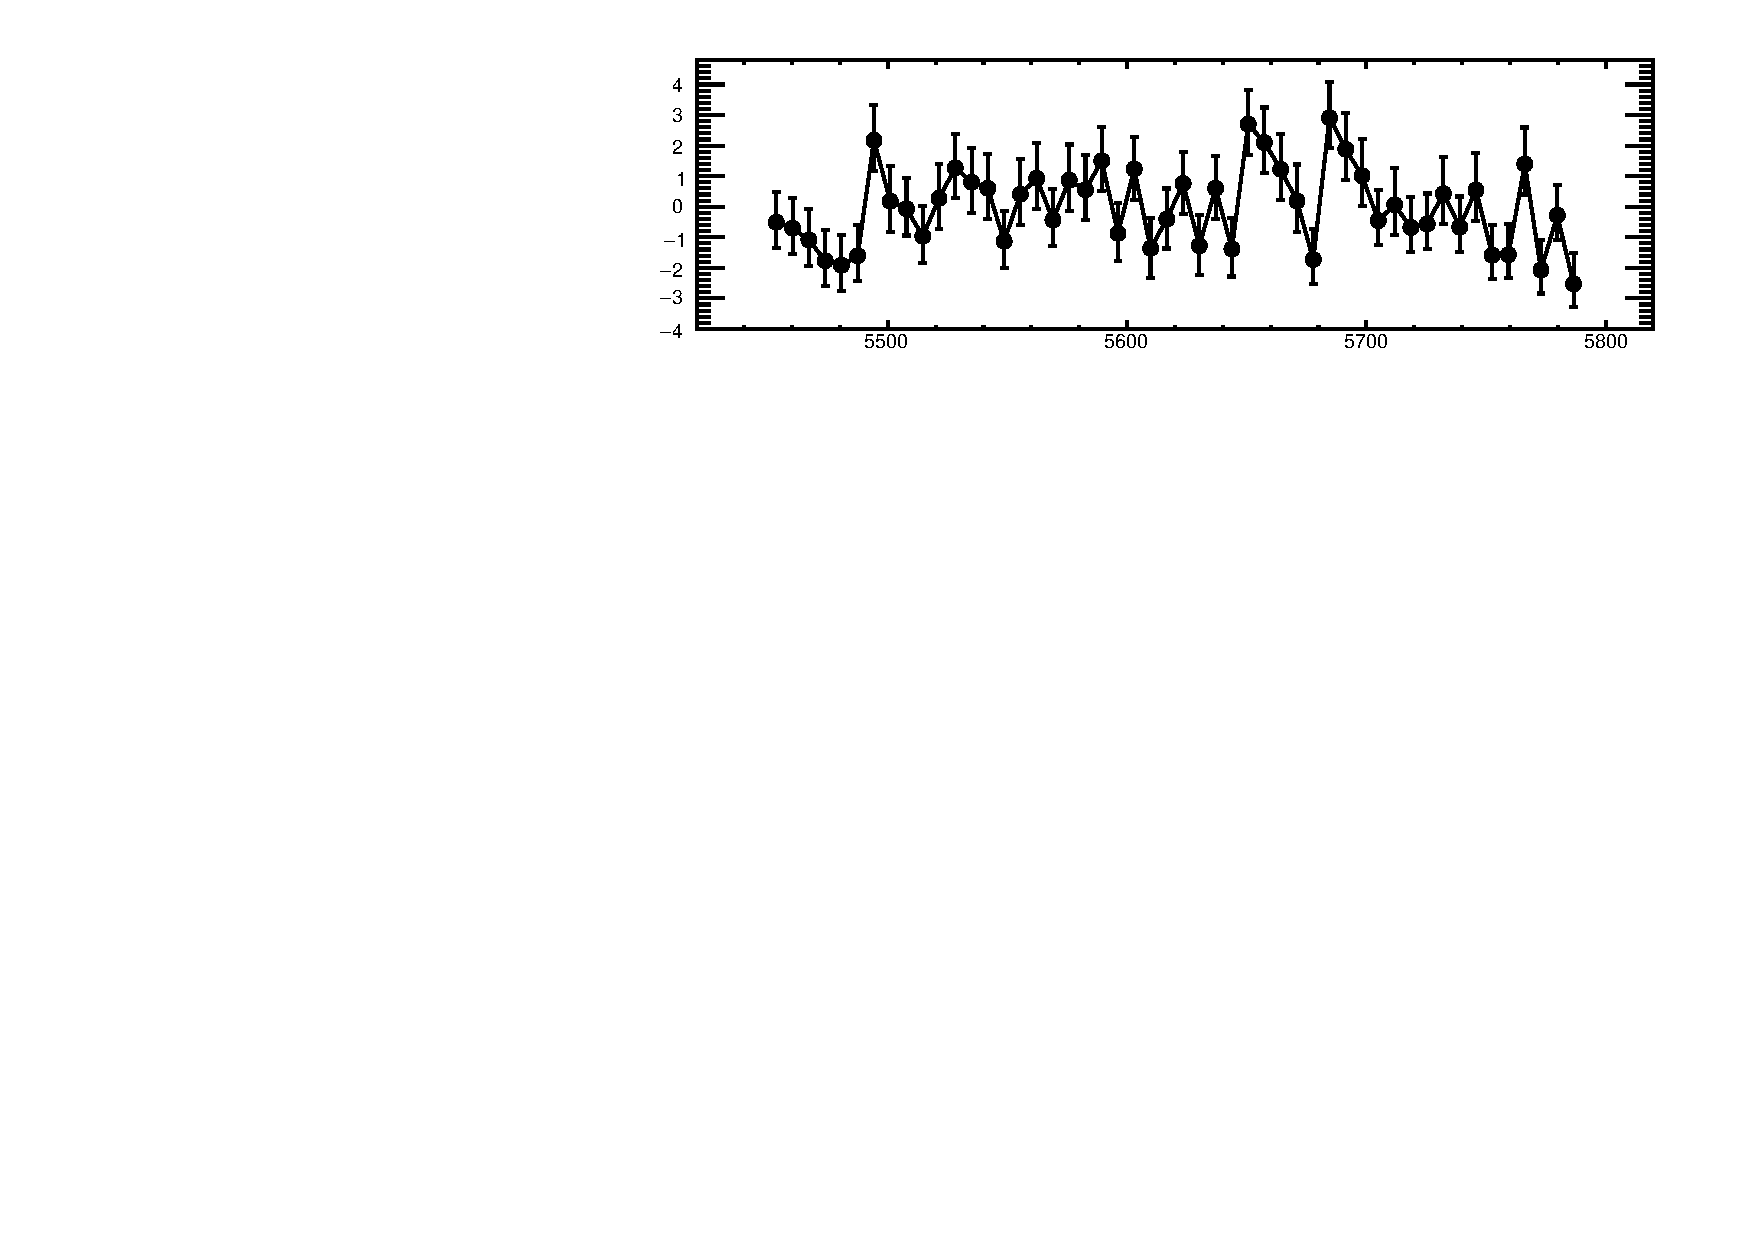
\includegraphics[scale=0.48]{Figures/05_open_charm/03_yiels/Data/Lb_LcDs_plot/Lb_LcDs_pull.pdf}%
\caption{Reconstructed mass distributions for \LbLcDs candidates. 
   A fit is overlaid, as described in the text. 
   The blue line is full fit, 
   the blue dashed line is the combinatorial background, 
   the green dashed line is the physical background, 
   the red line is the signal shape, 
   the pink dash line is \LbLckkpi background.}
\label{fig:MassFit_LbLcpi}
\end{figure}

\begin{table}[!btp]
\centering
\caption{Fit result of \LbLcDs mass spectrum in data sample.}
\vspace{0.2cm}
\label{tab:MassFit_LbLcpi}
\begin{tabular}{c c }\hline\hline
Parameter& Value \\\hline
$m_0$ (MeV/$c^2$)  & 5618.8 $\pm$ 0.3  \\
$n_{sig}$          & $ 2546.2 \pm 57.1  $  \\
$n_{phy bkg}$      & 477.7 $\pm$ 14.8\\
\hline\hline
\end{tabular}
\end{table}







